\documentclass[border=10pt]{standalone}

\usepackage{tikz}
\usepackage{tikzsymbols}
\usetikzlibrary{calc,patterns,shapes.geometric}

\def\centerarc[#1](#2)(#3:#4:#5){\draw[#1] ($(#2)+({#5*cos(#3)},{#5*sin(#3)})$) arc (#3:#4:#5);}

\begin{document}
	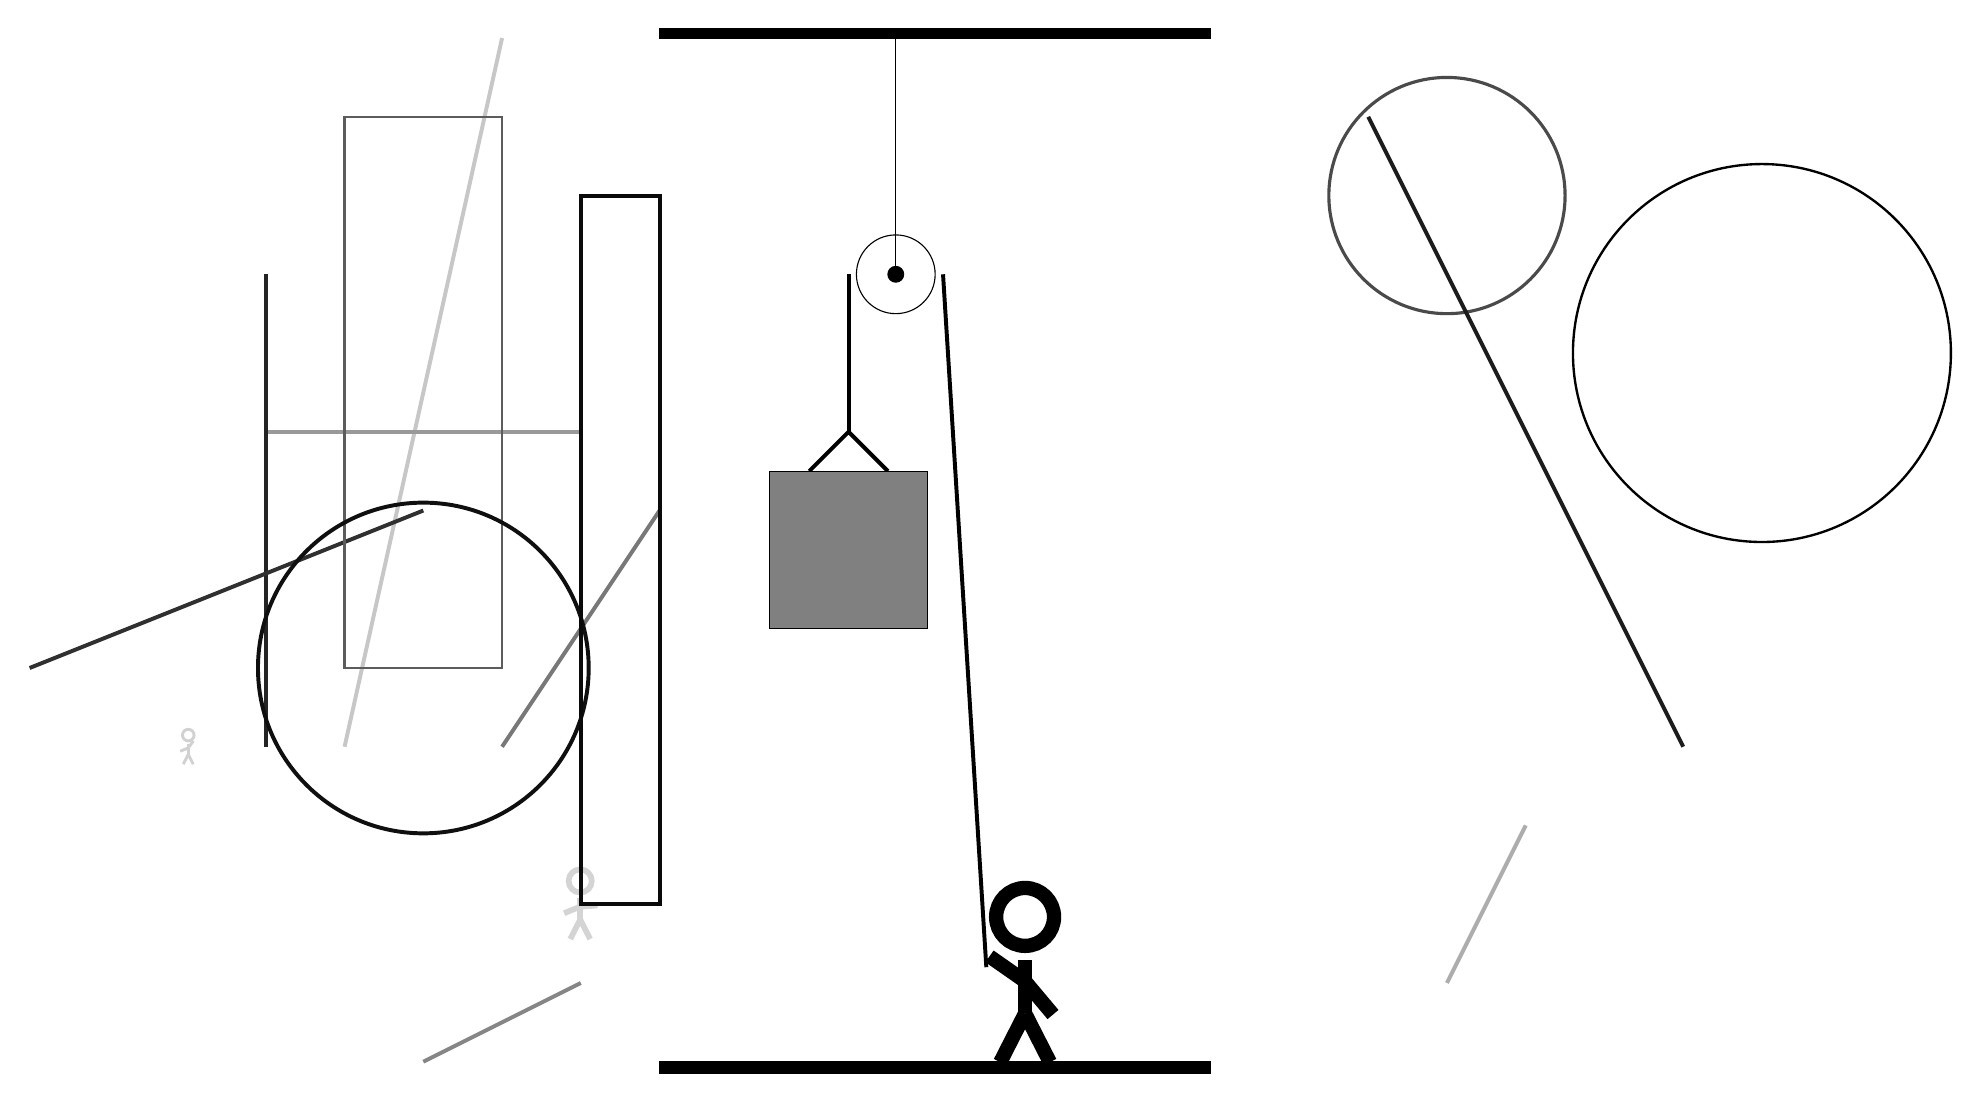
\begin{tikzpicture}
		%%%%% START %%%%%
		
		\draw[fill=black] (-2, 10) rectangle (5, 10.125);
		
		\draw (1, 7) circle (0.5);
		\draw[fill=black] (1, 7) circle (0.1);
		\draw (1, 10) -- (1, 7);
		
		\draw[line width=0.5mm] (-0.1, 4.5) -- (0.4, 5.0) -- (0.9, 4.5);
		\draw[fill=black!50] (-0.6, 4.5) rectangle (1.4, 2.5);
		
		\node[line width=0.3mm, color=black!17] at (-3, -1) {\Strichmaxerl[4][22][4]};
		
		\node[line width=0.2mm, color=black!18] at (-8, 1) {\Strichmaxerl[2][22][54]};
		\draw[line width=0.5mm, color=black!22](-6, 1) -- (-4, 10);
		\draw [line width=0.3mm, color=black!100](12, 6) circle (2.4);
		
		\draw[line width=0.5mm, color=black!32](8, -2) -- (9, 0);
		
		\draw[line width=0.5mm, color=black!40](-7, 5) -- (-3, 5);
		
		\draw[line width=0.5mm, color=black!86](-7, 1) -- (-7, 7);
		\draw[line width=0.5mm, color=black!81](-5, 4) -- (-10, 2);
		\draw[line width=0.3mm, color=black!64] (-4, 9) rectangle (-6, 2);
		
		\draw[line width=0.5mm, color=black!48](-5, -3) -- (-3, -2);
		
		\draw[line width=0.5mm, color=black!53](-4, 1) -- (-2, 4);
		\draw [line width=0.5mm, color=black!94](-5, 2) circle (2.1);
		\draw[line width=0.3mm, color=black!94] (-3, 4) rectangle (-3, 0);
		
		\draw[line width=0.5mm, color=black!96] (-2, 8) rectangle (-3, -1);
		\draw [line width=0.4mm, color=black!71](8, 8) circle (1.5);
		\draw[line width=0.5mm, color=black!89](7, 9) -- (11, 1);
		
		
		\draw[line width=0.5mm] (0.4, 7) -- (0.4, 5.0);
		\centerarc[line width=0.5mm](1, 7)(0:180:0.6);
		\draw[line width=0.5mm](1.6, 7) -- (2.15, -1.8);
		
		\node at (2.6, -1.9) {\Strichmaxerl[10][-35][-50]};
		
		\draw[fill=black] (-2, -3) rectangle (5, -3.15);
		
		%%%%% END %%%%%
	\end{tikzpicture}
\end{document}